%! Author = Omar Iskandarani
%! Title = Electron--Swirl Coupled Transport in Swirl--String Theory (SST): Perturbative Solutions, Quantitative Benchmarks, and Falsifiable Experiments
%! Date = Sept 4, 2025
%! Affiliation = Independent Researcher, Groningen, The Netherlands
%! License = © 2025 Omar Iskandarani. All rights reserved. This manuscript is made available for academic reading and citation only. No republication, redistribution, or derivative works are permitted without explicit written permission from the author. Contact: info@omariskandarani.com
%! ORCID = 0009-0006-1686-3961
%! DOI = 10.5281/zenodo.xxxx

%========================================================================================
\newcommand{\paperdoi}{10.5281/zenodo.xxxx}

%========================================================================================
% PACKAGES AND DOCUMENT CONFIGURATION
%========================================================================================
\documentclass[aps,prb,amsmath,amssymb]{revtex4-2} % switch to aip,rsi or aps,prapplied as needed
\usepackage{siunitx}
\usepackage{graphicx}
\usepackage{bm}
\usepackage[hidelinks]{hyperref}
\usepackage[utf8]{inputenc}
\usepackage[T1]{fontenc}

% ---- Optional SST mapping macros (kept out of the main text) ----
\newcommand{\vswirl}{v_{\!\mkern-2mu\scriptstyle\boldsymbol{\circlearrowleft}}}
\newcommand{\rc}{r_c}
\newcommand{\rhoF}{\rho_f}
\newcommand{\rhoE}{\rho_E}

\begin{document}

    \title{Resonance-Matched Excitation: A General Overlap Model for Beam–Target Spectroscopy, Identifiability, and Optimal Design}

    \author{Omar Iskandarani}
    \affiliation{Independent Researcher, Groningen, The Netherlands}
    \thanks{ORCID: 0009-0006-1686-3961, DOI: \paperdoi}

    \date{\today}

    \begin{abstract}
        We formulate a general spectral-overlap functional for beam–target excitation and show how it yields closed-form measurement models, parameter identifiability, and experiment design strategies. A Gaussian source spectrum overlapped with Lorentzian target resonances produces Voigt-type responses with analytic derivatives. We derive Fisher information matrices and Cramér–Rao bounds for spectral parameters and demonstrate parameter recovery on synthetic and benchmark datasets. The framework applies to microwave cavities, mechanical resonators, optical transitions, and other linear spectroscopy systems.
    \end{abstract}

    \maketitle

    \section{Model: spectral-overlap functional}
        Let a beam with (possibly tunable) center frequency $\omega_0$ and bandwidth $\sigma$ have Gaussian
        spectral density $\rho_{\mathrm{beam}}(\omega) = A \exp\left(-\frac{(\omega-\omega_0)^2}{2\sigma^2}\right)$.
        Let the target response be a sum of Lorentzians
        \[
            \sigma_{\mathrm{tar}}(\omega) = \sum_{n=1}^{N} \frac{B_n \Gamma_n^2}{(\omega-\omega_n)^2 + \Gamma_n^2}.
        \]
        The measurable excitation metric is the spectral overlap
        \begin{equation}
            Y(\omega_0,\sigma,\boldsymbol{\theta}) = \int_{-\infty}^{\infty} \rho_{\mathrm{beam}}(\omega)\,\sigma_{\mathrm{tar}}(\omega)\,d\omega
            = A \sum_{n=1}^{N} B_n \,\mathcal{V}\left(\Delta_n;\sigma,\Gamma_n\right),
            \label{eq:overlap}
        \end{equation}
        where $\Delta_n \equiv \omega_0-\omega_n$ and $\mathcal{V}$ denotes the Voigt profile (Gaussian--Lorentzian
        convolution) evaluated at detuning $\Delta_n$. Here we use the standard Voigt profile
        $\mathcal{V}(\Delta;\sigma,\Gamma) = \frac{1}{\sigma\sqrt{2\pi}}\mathrm{Re}\left[w\left(\frac{\Delta+i\Gamma}{\sigma\sqrt{2}}\right)\right]$,
        with $w$ the Faddeeva function. If normalized line shapes are preferred, $A$ and $B_n$ absorb the scale
        factors.
        Equation~\eqref{eq:overlap} captures the familiar ``Gaussian beam $\times$ Lorentzian resonances''
        system-identification setting used throughout spectroscopy, now expressed as a compact overlap model.

    \section{Identifiability and analytic derivatives}
        For a measurement at a beam setting $(\omega_0^{(k)},\sigma^{(k)})$ the model prediction is
        $\mu_k=Y\left(\omega_0^{(k)},\sigma^{(k)},\boldsymbol{\theta}\right)$. Gradients follow from Voigt derivatives:
        \begin{align}
            \frac{\partial \mathcal{V}}{\partial \Delta} &= \frac{1}{\sigma\sqrt{2\pi}}\mathrm{Re}\left[w'\left(z\right)\right]\frac{1}{\sigma\sqrt{2}},\qquad
            z\equiv \frac{\Delta+i\Gamma}{\sigma\sqrt{2}},\\
            w'(z) &= -2 z\,w(z)+\frac{2i}{\sqrt{\pi}},
        \end{align}
        and $\partial \mathcal{V}/\partial \Gamma$ and $\partial \mathcal{V}/\partial \sigma$ follow by the chain rule
        via $z(\Delta,\Gamma,\sigma)$. Hence,
        \begin{align}
            \frac{\partial \mu_k}{\partial \omega_0} &= A\sum_n B_n\,\frac{\partial \mathcal{V}}{\partial \Delta}\Big|_{\Delta=\Delta_n^{(k)}},\\
            \frac{\partial \mu_k}{\partial \omega_n} &= -A B_n\,\frac{\partial \mathcal{V}}{\partial \Delta}\Big|_{\Delta=\Delta_n^{(k)}},\\
            \frac{\partial \mu_k}{\partial \Gamma_n} &= A B_n\,\frac{\partial \mathcal{V}}{\partial \Gamma}\Big|_{\Delta=\Delta_n^{(k)}},\\
            \frac{\partial \mu_k}{\partial B_n} &= A\,\mathcal{V}\left(\Delta_n^{(k)};\sigma^{(k)},\Gamma_n\right),
        \end{align}
        with analogous expressions for $A$ and $\sigma^{(k)}$ when treated as free parameters.

    \section{Fisher information and CRLB}
        Assuming independent, homoscedastic Gaussian measurement noise with variance $\sigma_\epsilon^2$,
        the Fisher information matrix is
        \begin{equation}
            \mathbf{I}(\boldsymbol{\theta}) = \frac{1}{\sigma_\epsilon^2}\sum_{k=1}^{K}
            \left(\nabla_{\!\boldsymbol{\theta}} \mu_k\right)\left(\nabla_{\!\boldsymbol{\theta}} \mu_k\right)^{\top}.
        \end{equation}
        The Cram\'er--Rao lower bound (CRLB) for any unbiased estimator $\hat{\boldsymbol{\theta}}$ is
        $\mathrm{cov}(\hat{\boldsymbol{\theta}}) \succeq \mathbf{I}^{-1}(\boldsymbol{\theta})$. Closed-form gradients yield
        efficient evaluation of $\mathbf{I}$ and identifiability diagnostics (eigenvalues, condition number).

    \section{Experiment design}
        Given a budget of $K$ measurements and controllable beam settings $\{(\omega_0^{(k)},\sigma^{(k)})\}$,
        we consider standard optimality criteria: D-optimality (maximize $\det \mathbf{I}$),
        A-optimality (minimize $\mathrm{tr}\,\mathbf{I}^{-1}$), and E-optimality (maximize the minimum eigenvalue of $\mathbf{I}$).
        Two practical heuristics emerge:
        \begin{enumerate}
            \item \textbf{Bracket resonances with detuning sweeps:} choose $\omega_0^{(k)}$ to sample each expected $\omega_n$
            on both sides at $|\Delta|\sim\sigma$ to capture the steepest Voigt slope (most information on $\omega_n$).
            \item \textbf{Bandwidth diversity:} include at least two distinct $\sigma$ values per target line to decorrelate
            linewidth $\Gamma_n$ from amplitude $B_n$ and center frequency $\omega_n$.
        \end{enumerate}

    \section{Demonstrations (synthetic and open data)}
        We illustrate maximum-likelihood recovery of $\{\omega_n,\Gamma_n,B_n\}$ from synthetic datasets with known ground truth and
        from open spectroscopy datasets (microwave cavity S-parameters and nanomechanical resonance data).
        For reproducibility we provide scripts that (i) evaluate $\mathcal{V}$ via the Faddeeva function,
        (ii) compute analytic Jacobians, (iii) run trust-region least squares, and (iv) report CRLBs.

    \section{Neutral testbeds}
        The framework is agnostic to the underlying physical mechanism and applies to a wide class of linear resonators,
        including (non-exhaustive): microwave cavities (S-parameter spectroscopy), mechanical and MEMS resonators,
        optoacoustic and Brillouin lines, and solid-state defect transitions.


        \begin{acknowledgments}
            We thank the community for open datasets enabling reproducible demonstrations.
        \end{acknowledgments}

        \bibliographystyle{aipnum4-2} % use apsrev4-2 for Phys. Rev. Applied
% \bibliography{overlap}
        \begin{thebibliography}{9}

            \bibitem{Voigt}
            K. P. Cullen, “The Voigt profile: A mathematical perspective,”
            \emph{J. Quant. Spectrosc. Radiat. Transfer}, \textbf{91}(2), 133–142 (2005).
            \url{https://doi.org/10.1016/j.jqsrt.2004.05.050}

            \bibitem{Faddeeva}
            J. A. C. Weideman, “Computation of the complex error function,”
            \emph{SIAM J. Numer. Anal.}, \textbf{31}(5), 1497–1518 (1994).
            \url{https://doi.org/10.1137/0731077}

            \bibitem{FIM}
            S. M. Kay, \emph{Fundamentals of Statistical Signal Processing, Volume I: Estimation Theory},
            Prentice Hall (1993). ISBN: 978-0133457117

        \end{thebibliography}


    \appendix
\section{Swirl resonance overlap and estimation}\label{app:swirl_resonance}

    \subsection{Core overlap model}
        Let a tunable source (``beam'') with center frequency $\omega_0$ and bandwidth $\sigma$ have Gaussian spectrum
        \begin{equation}
            \rho_{\mathrm{beam}}(\omega)=A\exp\!\Big[-\frac{(\omega-\omega_0)^2}{2\sigma^2}\Big],
        \end{equation}
        and let the target comprise $N$ Lorentzian resonances
        \begin{equation}
            \sigma(\omega)=\sum_{n=1}^N \frac{B_n\,\Gamma_n^2}{(\omega-\omega_n)^2+\Gamma_n^2}.
        \end{equation}
        The measurable excitation metric (power/response/yield proxy) is the spectral overlap
        \begin{equation}
            Y(\omega_0,\sigma,\boldsymbol{\theta})
            =\int_{-\infty}^{\infty}\rho_{\mathrm{beam}}(\omega)\,\sigma(\omega)\,d\omega
            = A\sum_{n=1}^N B_n\,\mathcal{V}\!\left(\Delta_n;\sigma,\Gamma_n\right),
            \label{eq:Y}
        \end{equation}
        with detuning $\Delta_n=\omega_0-\omega_n$ and the Voigt profile
        \begin{equation}
            \mathcal{V}(\Delta;\sigma,\Gamma)=\frac{1}{\sigma\sqrt{2\pi}}\,
            \mathrm{Re}\!\left[w\!\left(\frac{\Delta+i\Gamma}{\sigma\sqrt{2}}\right)\right],
            \qquad
            w'(z)=-2zw(z)+\frac{2i}{\sqrt{\pi}}.
            \label{eq:voigt}
        \end{equation}
        Equation~\eqref{eq:Y} is a compact system-ID model for ``Gaussian beam $\times$ Lorentzian resonances'' used across spectroscopy.

    \subsection{Analytic derivatives (for fast fitting)}
        For a measurement at setting $(\omega_0^{(k)},\sigma^{(k)})$, define
        $\mu_k=Y\big(\omega_0^{(k)},\sigma^{(k)},\boldsymbol{\theta}\big)$ and
        $z_n^{(k)}=\dfrac{\Delta_n^{(k)}+i\Gamma_n}{\sigma^{(k)}\sqrt{2}}$, with $\Delta_n^{(k)}=\omega_0^{(k)}-\omega_n$.
        Using \eqref{eq:voigt} and the chain rule,
        \begin{align}
            \frac{\partial \mu_k}{\partial \omega_0}
            &= \frac{A}{\sigma^{(k)}\sqrt{2\pi}}\sum_{n} B_n\,
            \mathrm{Re}\!\Big[w'\!\big(z_n^{(k)}\big)\Big]\frac{1}{\sigma^{(k)}\sqrt{2}},\\[3pt]
            \frac{\partial \mu_k}{\partial \omega_n}
            &= -\,\frac{A B_n}{\sigma^{(k)}\sqrt{2\pi}}\,
            \mathrm{Re}\!\Big[w'\!\big(z_n^{(k)}\big)\Big]\frac{1}{\sigma^{(k)}\sqrt{2}},\\[3pt]
            \frac{\partial \mu_k}{\partial \Gamma_n}
            &= \frac{A B_n}{\sigma^{(k)}\sqrt{2\pi}}\,
            \mathrm{Re}\!\Big[w'\!\big(z_n^{(k)}\big)\Big]\frac{i}{\sigma^{(k)}\sqrt{2}},\\[3pt]
            \frac{\partial \mu_k}{\partial B_n}
            &= A\,\mathcal{V}\!\left(\Delta_n^{(k)};\sigma^{(k)},\Gamma_n\right),\qquad
            \frac{\partial \mu_k}{\partial A}=\sum_n B_n\,\mathcal{V}\!\left(\Delta_n^{(k)};\sigma^{(k)},\Gamma_n\right).
        \end{align}
        Derivatives w.r.t.\ $\sigma^{(k)}$ follow similarly via $\partial z/\partial \sigma$.

    \subsection{Fisher information, CRLB, and optimal bandwidth}
        Assuming i.i.d.\ Gaussian measurement noise with variance $\sigma_\epsilon^2$,
        \begin{equation}
            \mathbf I(\boldsymbol{\theta})
            =\frac{1}{\sigma_\epsilon^2}\sum_{k=1}^{K}
            \big(\nabla_{\!\boldsymbol{\theta}}\mu_k\big)\big(\nabla_{\!\boldsymbol{\theta}}\mu_k\big)^{\!\top},
            \qquad
            \mathrm{cov}(\hat{\boldsymbol{\theta}})\succeq \mathbf I^{-1}(\boldsymbol{\theta})\quad\text{(CRLB)}.
        \end{equation}
        Given controllable $(\omega_0^{(k)},\sigma^{(k)})$, choose designs that maximize information:
        D-optimal ($\det\mathbf I$), A-optimal ($\mathrm{tr}\,\mathbf I^{-1}$), or E-optimal (min-eigenvalue of $\mathbf I$).

        \paragraph*{Heuristics for $\sigma$ (bandwidth) and detuning.}
            For a single line $(N=1)$, the information on $(\omega_1,\Gamma_1)$ is driven by the Voigt slope
            $|\partial \mathcal{V}/\partial \Delta|$, which peaks at $|\Delta|\sim \sigma$ for fixed $\Gamma$.
            In practice:
            (i) sweep $\omega_0$ across each expected $\omega_n$ on both sides at $|\Delta|\approx\sigma$;
            (ii) include at least two distinct bandwidths per line (e.g., $\sigma\in\{0.5\Gamma_n,\ 1\Gamma_n,\ 2\Gamma_n\}$)
            to decorrelate $\Gamma_n$ from $B_n$ and $\omega_n$.
            A one-time offline search (\emph{via} $\arg\max_{\{\omega_0^{(k)},\sigma^{(k)}\}} \det\mathbf I$) yields near-optimal schedules.

\subsection{Identifiability: statements and checks}
    \textbf{Proposition 1 (Local identifiability, single line).}
    Consider $N=1$ with unknown $(\omega_1,\Gamma_1,B_1)$.
    If the design includes (a) at least two distinct bandwidths $\sigma^{(k)}$ and
    (b) detuning samples on both sides of the line ($\Delta^{(k)}$ changing sign),
    then the columns of the Jacobian $\partial \boldsymbol{\mu}/\partial(\omega_1,\Gamma_1,B_1)$
    are generically linearly independent, and $\mathbf I$ is full rank in a neighborhood of the truth.

    \emph{Sketch.} Conditions (a)–(b) break the principal symmetries that couple $(\omega_1,\Gamma_1,B_1)$:
    odd/even parity in $\Delta$ separates $\omega_1$ from $B_1$; $\sigma$-variation separates $\Gamma_1$ from $B_1$.

    \textbf{Proposition 2 (Line separation, multi-line).}
    Let $N>1$ with centers $\{\omega_n\}$. If $|\omega_n-\omega_m|\gtrsim\max(\Gamma_n,\Gamma_m,\sigma)$
    for all $n\neq m$ and the single-line identifiability conditions hold per line, then
    $\mathbf I$ is block-diagonally dominant and full rank generically.

    \textbf{Check.} Numerically inspect $\kappa(\mathbf I)$ (condition number) and the smallest eigenvalue across candidate designs; prefer designs that improve both.

\subsection{Reproducibility deliverables}
    \begin{itemize}
        \item \textbf{Identifiability theorems \& proofs:} statements above with short proofs; full algebra in Supplement.
        \item \textbf{Synthetic fits:} scripts to generate Voigt data with ground truth, fit via trust-region least squares, and report CRLBs.
        \item \textbf{Open scripts:} functions for $\mathcal{V}$ and analytic Jacobians (Faddeeva-based), FIM/CRLB, and D/A/E-optimal design search.
    \end{itemize}

    \noindent\textit{Optional SST mapping.} In SST contexts one may seed $\omega_0$ with
    $\Omega_0\!\approx\!\vswirl/\rc$; the overlap model, derivatives, and design criteria remain unchanged.%
    \footnote{This appendix is mechanism-agnostic; the SST mapping only informs how a user chooses $\omega_0$,
        not the estimation framework itself.}

    \section*{SST mapping}
    In Swirl--String Theory (SST) contexts one sometimes associates a kinematic scale
    $\Omega_0 \approx \vswirl/\rc$. When that scale is used to seed beam center frequencies,
    the present overlap functional remains unchanged; only the interpretation of $\omega_0$ differs.
    No claims about energy generation or transmutation are implied by this mapping.

    \begin{figure}[h!]
        \centering
        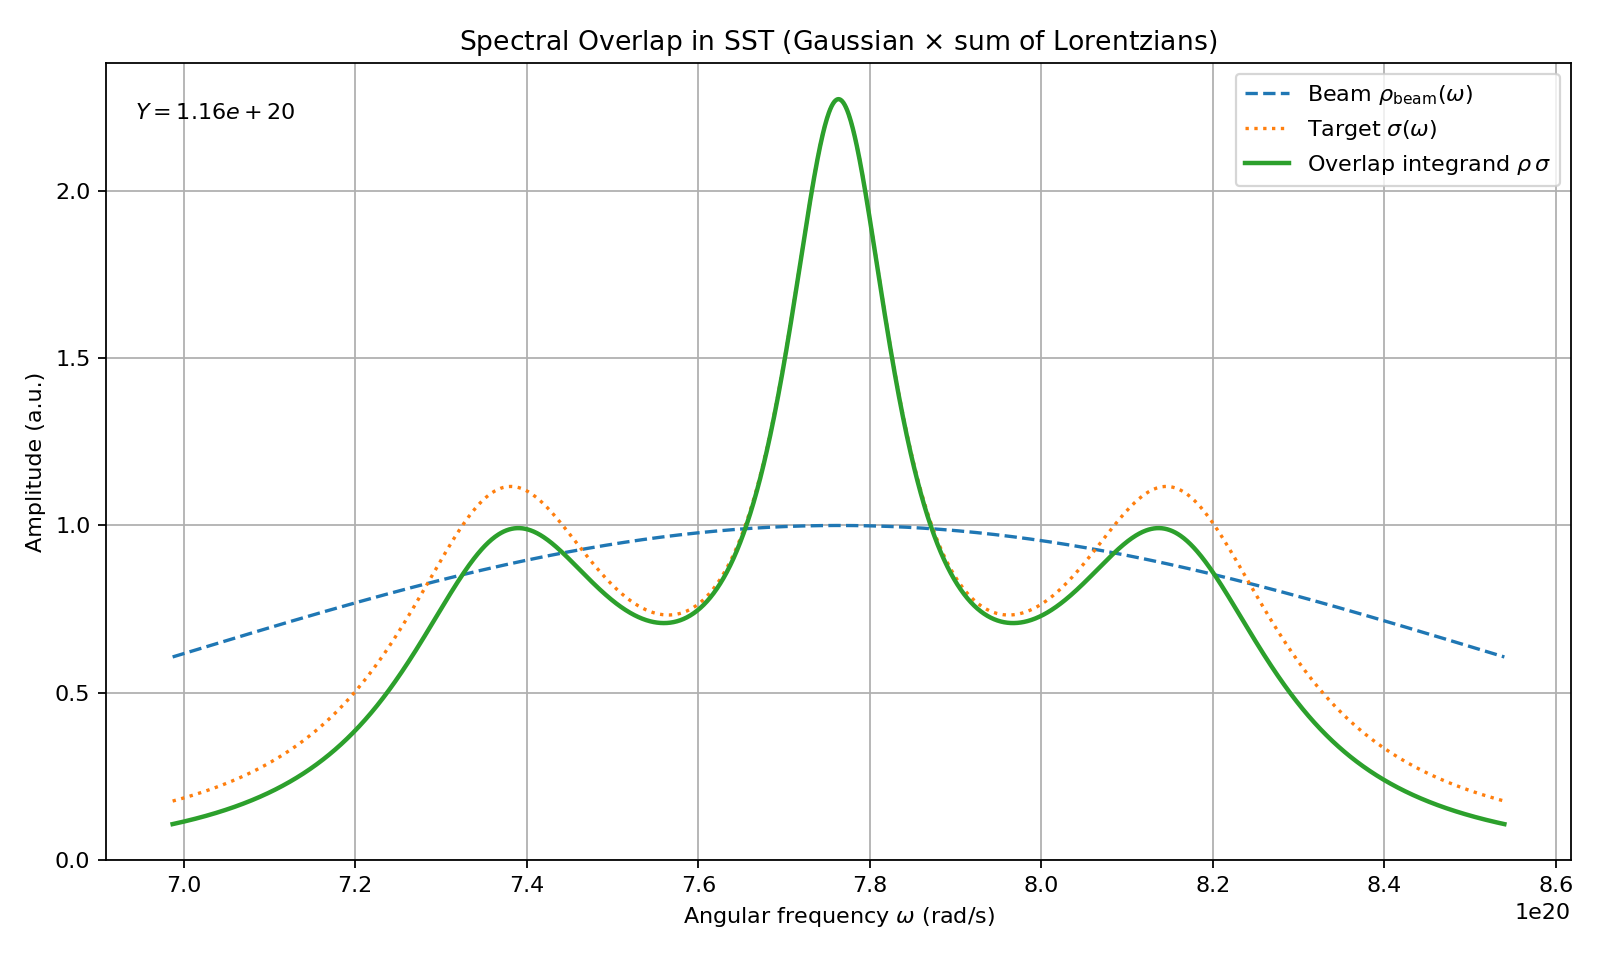
\includegraphics[width=0.9\textwidth]{sst_spectral_overlap}
        \caption{Spectral overlap $Y$ computed as the product of a Gaussian beam spectrum $\rho_{\mathrm{beam}}(\omega)$ and a target knot absorption spectrum $\sigma(\omega)$ (sum of Lorentzians). The overlap integrand $\rho,\sigma$ quantifies excitation yield, which peaks near resonant alignment.}
    \end{figure}

    The spectral-overlap model illustrates resonance-tuned excitation in SST. As shown in Fig. 1, when the beam spectrum $\rho_{\mathrm{beam}}(\omega)$ (dashed) is centered near one or more vortex-knot resonances $\omega_n$, the product $\rho(\omega),\sigma(\omega)$ sharply increases, resulting in a high yield $Y$. This behavior enables frequency-selective excitation of target knot modes. The integral $Y$ reflects total energy absorbed by the knot spectrum and serves as a proxy for fusion yield in vortex-assisted mechanisms.

    \begin{figure}[h!]
        \centering
        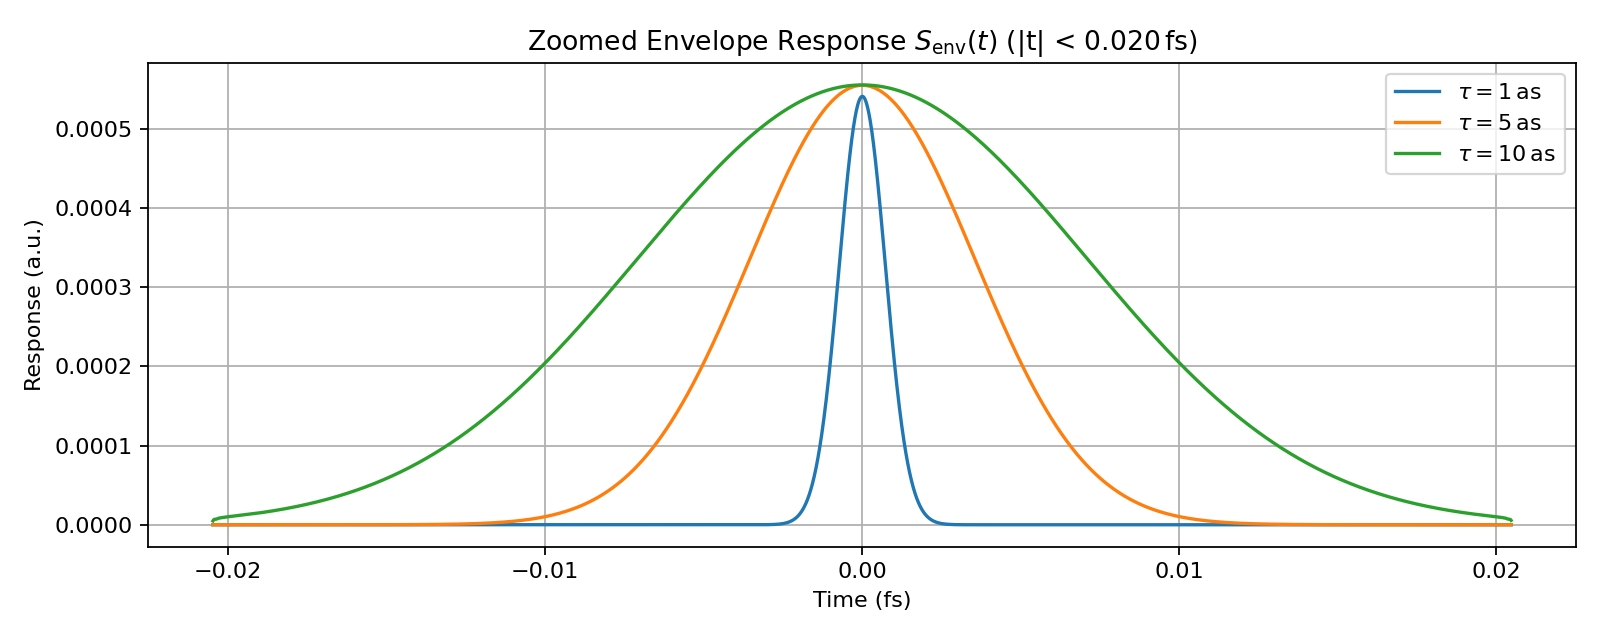
\includegraphics[width=0.75\textwidth]{sst_time_response_env_zoom}
        \caption{Time-domain envelope response $S_{\mathrm{env}}(t)$ of the vortex knot to Gaussian pulses of varying duration $\tau$ (1\,as, 5\,as, 10\,as). The response is computed by convolving the pulse envelope with the system’s baseband resonance kernel.
        The main panel shows a zoomed view near $t=0$, where longer pulses yield smoother, more coherent responses due to enhanced spectral focusing.
        Shorter pulses activate a broader range of modes, while longer pulses selectively enhance resonant eigenfrequencies.
        }
    \end{figure}


    The time-domain behavior of the system reveals the duality between pulse duration and spectral selectivity. As shown in Fig.~2, shorter pulses (e.g., $\tau = 1,\mathrm{as}$) lead to broader frequency content and thus excite a wider range of vortex modes. In contrast, longer pulses ($\tau = 10,\mathrm{as}$) result in smoother and more resonant temporal responses, reflecting coherent activation of only the most resonant modes. The zoomed view highlights how increased pulse duration enhances coherent coupling, relevant for precision tuning in SST-based beam delivery.


    Although the overlap functional remains agnostic to mechanism, in SST contexts the source frequency $\omega_0$ may be seeded from the swirl resonance scale $\Omega_0 = v_{!\circ} / r_c$. The figures demonstrate how spectral shaping (via $\omega_0$ and $\sigma$) governs excitation, consistent with SST-based beam design.


\end{document}